\documentclass[12pt, aspectratio=169]{beamer}

\usetheme{Copenhagen}
\usefonttheme{professionalfonts}
\setbeamertemplate{navigation symbols}{}
% \setbeamertemplate{page number in head/foot}[totalframenumber]
\setbeamertemplate{page number in head/foot}{
  \usebeamerfont{page number in head/foot}
  \usebeamercolor[fg]{page number in head/foot}
  \LR{\insertframenumber\ /\ \inserttotalframenumber}
}

%Packages-------------------------------------
\usepackage[svgnames]{xcolor}
\usepackage{amsmath, amsthm, amscd, amsfonts, amssymb}
\usepackage{tikz}
\usetikzlibrary{arrows.meta, positioning}
% \usepackage{tikz}
% \usepackage{setspace}
% \usepackage{wasysym}
% \usepackage{framed}
% \usepackage{enumitem}
% \usepackage{graphics}
% \usepackage{graphicx}
% \usepackage{cite}
% \DeclareGraphicsExtensions{.pdf,.png,.jpg}
\usepackage{mathtools}
% \usepackage{lipsum}
% \usepackage{perpage}
% \usepackage{bussproofs}
% \usepackage{listings}

\usepackage{listings}

\lstdefinelanguage{Coq}{
  keywords={Inductive, Type},
  morekeywords=[2]{base, arrow},
  sensitive=true,
  morecomment=[s]{(*}{*)},
  morestring=[b]"
}

\lstset{
  language=Coq,
  basicstyle=\ttfamily\small,
  keywordstyle=\color{blue},
  keywordstyle=[2]\color{teal},
  commentstyle=\color{gray},
  frame=single,
  columns=fullflexible
}

% \tikzstyle{vertex}=[circle, draw, inner sep=0pt, minimum size=6pt]
% \newcommand{\vertex}{\node[vertex]}
% \usepackage{relsize}
% \usepackage{bookmark}
\usepackage{xepersian}
\settextfont{XB Zar}
\setlatintextfont{Times New Roman}
% \MakePerPage[1]{LTRfootnote}
% \MakePerPage[1]{footnote}
% \linespread{1.3}

\title{صوری‌سازی ترجمه حذف وابستگی در سیستم‌های نوع محض لایه‌ای}

\author{حسین مددی}

\institute{
  استاد راهنما\\
  {\small دکتر مجید علی‌زاده}\\
  {\hfil}\\
  سمینار کارشناسی ارشد\\
  دانشکده ریاضی، آمار و علوم‌ کامپیوتر\\
  دانشکدگان علوم\\
  دانشگاه تهران
}

\date{\small زمستان ۱۴۰۴}

\begin{document}

\maketitle

\begin{frame}{مسئله اصلی}

\textbf{مسئله نرمال‌سازی (حدس \lr{BGK}\footnote{\lr{Barendregt–Geuvers–Klop}})}\\
در هر سیستم نوع محض\footnote{\lr{PTS}}؛
نرمال‌سازی ضعیف
\pmb{$\overset{?}{\impliedby}$}
نرمال‌سازی قوی
\hfil\\
\hfil\\
{\small
  \begin{itemize}
      \item \textbf{فرم نرمال ($\mathrm{NF}$):} عبارتی که قابل کاهش نباشد.
      \item \textbf{نرمال‌سازی ضعیف ($\mathrm{WN}$):} وجود مسیر کاهش به فرم نرمال برای هر عبارت نوع‌پذیر.\\
      \begin{align*}
        A \to \dots \to N
      \end{align*}
      \item \textbf{نرمال‌سازی قوی ($\mathrm{SN}$):} عدم وجود دنباله کاهش نامتناهی برای هر عبارت نوع‌پذیر.\\
      \begin{align*}
        \dots \to B \to \dots
      \end{align*}
  \end{itemize}
}

\end{frame}

\begin{frame}{چرا این مسئله دشوار است؟}

در سیستم‌های وابسته؛

\begin{columns}

\begin{column}{0.5\textwidth}
\hfil{}\\
\begin{itemize}
  \item انواع به عبارات وابسته‌اند.
  \item کاهش روی نوع اثر می‌گذارد.
  \item جانشینی بسیار ظریف و حساس می‌شود.
\end{itemize}   
\end{column}

\begin{column}{0.5\textwidth}

\begin{center}
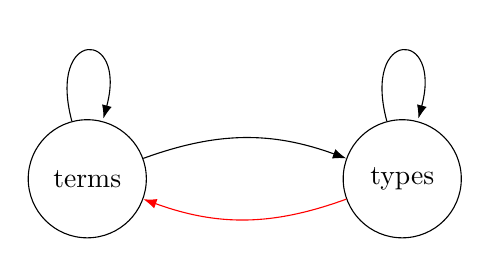
\begin{tikzpicture}[
    node distance=4cm,
    every node/.style={draw, circle, minimum size=1.5cm},
    >={Latex}
]

\node (terms) {terms};
\node (types) [right of=terms] {types};

% self loops
\draw[->] (terms) edge[loop above] (terms);
\draw[->] (types) edge[loop above] (types);

% cross edges
\draw[->] (terms) to[bend left=20] (types);
\draw[->, red] (types) to[bend left=20] (terms);

\end{tikzpicture}
\end{center}

\end{column}

\end{columns}

\end{frame}

\begin{frame}[t]{سیستم \lr{Nathan Mull}}

\begin{columns}[T]
  
\begin{column}{0.83\textwidth}
  
\begin{flushright}
  
\textbf{سیستم‌های نوع محض لایه‌ای}\\

\begin{align*}
\mathrm{TPTS} \subset \mathrm{PTS}
\end{align*}

{\small
  \begin{itemize}
    \item اختصاص درجه به انواع و عبارات
    \item محدودسازی وابستگی بین درجات
  \end{itemize}
}


\begin{align*}
\mathrm{TPTS} \in \mathrm{WN} \pmb{\overset{?}{\implies}} \mathrm{TPTS} \in \mathrm{SN}
\end{align*}

\end{flushright}

\end{column}

\begin{column}{0.17\textwidth}

\includegraphics[scale=0.13]{mull.jpeg}
\end{column}

\end{columns}

\end{frame}

\begin{frame}{ترجمه \lr{Nathan Mull}}

\textbf{ترجمه حذف وابستگی}

تابعی که هر سیستم نوع محض لایه‌ای را به نسخه غیروابسته آن نگاشت می‌کند.

\begin{align*}
\lambda_S &\overset{f}{\longrightarrow} \lambda_{S^*} &\text{تابع ترجمه}\\
\lambda_{S^*} \in \mathrm{SN} &\implies \lambda_S \in \mathrm{SN} &\text{لم}\\
\lambda_S &\in \mathrm{SN} &\text{نتیجه}
\end{align*}

\textbf{نتیجه}\\
حدس \lr{BGK} برای سیستم‌های نوع محض لایه‌ای، برقرار است.

\end{frame}

\begin{frame}{هدف پایان‌نامه من}

\textbf{صوری‌سازی سیستم، ترجمه و اثبات نرمال‌سازی در \lr{COQ}}\\
\hfil{}\\
چرا؟\\

\begin{columns}
  
\begin{column}{0.5\textwidth}
\begin{center}
{\small
  \begin{itemize}
    \item ظرافت بالای اثبات‌های نرمال‌سازی
    \item جلوگیری از شکاف‌های پنهان
    \item رسیدن به کتاب‌خانه‌ای قابل توسعه و گسترش
  \end{itemize}
}
\end{center}
\end{column}

\begin{column}{0.5\textwidth}
\begin{center}

\includegraphics[scale=0.1]{coq.png}
\end{center}
\end{column}

\end{columns}

\end{frame}

\begin{frame}{کارهای انجام‌شده}

\textbf{فصل‌های اول و دوم}  

\begin{columns}
  
\begin{column}{0.5\textwidth}
\begin{center}
{\small
  \begin{itemize}
  \item بیان مفاهیم و تعاریف اولیه پیش‌نیاز
  \item صورت‌بندی سیستم‌های نوع محض لایه‌ای
  \item تعریف دقیق ترجمه حذف وابستگی
  \item ارائه اثبات ریاضی برای لم‌های اصلی
  \end{itemize}
}
\end{center}
\end{column}

\begin{column}{0.5\textwidth}
\begin{center}
\frame{
\includegraphics[scale=0.17]{done.png}}
\end{center}
\end{column}

\end{columns}

\end{frame}

\begin{frame}[fragile]
  \frametitle{کارهای باقی‌مانده}

\textbf{فصل‌‌های سوم و چهارم}\\

\begin{columns}
  
\begin{column}{0.45\textwidth}
\begin{RTL}
پیاده‌سازی موارد زیر در \lr{COQ}:
\end{RTL}
\begin{center}
{\small
  \begin{itemize}
  \item سیستم نوع محض لایه‌ای
  \item توابع ترجمه حذف وابستگی
  \item صوری‌سازی خواص و لم‌ها
  \item صوری‌سازی قضیه اصلی
  \end{itemize}
}
\end{center}
\end{column}

\begin{column}{0.55\textwidth}
\begin{LTR}  
\begin{lstlisting}[basicstyle=\ttfamily\footnotesize]
Inductive type : Type :=
         | base : type
         | arrow : type -> type -> type.
\end{lstlisting}
\end{LTR}
\end{column}

\end{columns}

\end{frame}

\end{document}
